%%%%%%%%%%%%%%%%%%%%%%%%%%%%%%%%%%%%%%%%%%%%%%%%%%%%%%%%%%%
%%%%%%%%%%%%%%%%%%%%%%%%%%%%%%%%%%%%%%%%%%%%%%%%%%%%%%%%%%%
\subsection{EMMA}

%%%%%%%%%%%%%%%%%%%%%%%%%%%%%%%%%%%%%%%%%%%%%%%%%%%%%%%%%%%%%%%%%%%%%%%%%%%%%%%%%%%%%%%%5
%\subsubsection{all samples}
A total of 30 recipes (see appendix \ref{sec:app-emma}) have been investigated in 
five iterations ($t = 0, \dots, 4$) of the algorithm. 
Where the first generation encompassed 10 particles and each subsequent generation encompassed 5 particles. 
The best recipes for each generation can be seen in table \ref{tab:emma-Gb}. 
The experiments for generation 5 where not executed but 
predictions were alread made
with the information from the previous generations. 
%%% BEST
The best sample predicted by the algorithm is experiment number 13 with 
lowest solution concentration, second highest layer count, lowest \gls{db} velocity and temperature, 
and lowest calcination heating rate and temperature. 

\begin{table}[htb]
	\centering
    \caption{Global best per generation}
	\label{tab:emma-Gb}
	\begin{tabular}{cccccccc}
        \hline\hline
        generation  &enr &conc &layr &$v_{DB}$ &$T_{DB}$ &$v_{cal}$ &$T_{cal}$\\
        \hline
     1   &1       &2    &4   &10   &40  &120  &300\\
     2   &5       &2    &6   &10   &40  &120  &300\\
     3   &2947    &4    &6   &16   &80 &1080  &300\\
     4   &2405    &2    &6   &10   &40 &1080  &300\\
     5   &13      &2   &10   &10   &40  &120  &300\\
    \hline\hline
	\end{tabular}
\end{table}

\begin{table}
	\centering
    \caption{Predicted G} 
    \label{tab:emma-pred-G}
    \begin{tabular}{cccccc}
        \hline\hline
    enr     &1st gen     &2nd gen        &3rd gen        &4th gen        &5th gen\\
        \hline
    1       &1.214185    &       &       &       &38.7962       \\
    5       &       &4.196626       &       &       &25.47335       \\
    2947    &       &       &10.9594    &       &10.9594       \\
    2405    &       &       &       &20.04962   &25.47335       \\
    13      &       &       &       &       &24.87178   \\
        \hline\hline
    \end{tabular}
\end{table}

%%% OVER TIME 
The only clear trend from table \ref{tab:emma-Gb} is the layer count, which rises with the generations. 
The remaining input variables remained more or less the same except for the 3rd generation. 
%
In table \ref{tab:emma-pred-G} it can be seen that $G$ as predicted 
by the 5th generation by the prediction function lowered with each iteration, 
except for sample 2947, which wasn't predicted but measured. 
This shows that the easiest part of the algorithm, the selection of the optimum 
from predicted values works as expected. 
% and that the predictions included more lower values over time
%
The predicted $G$ for each generation's best as predicted 
by the very generation would increase with each iteration (see table \ref{tab:emma-pred-G}). 
This indicates an underestimation of the $G$ at the beginning and a correction with time. 
%The reason for is probably a 
The underestimation probably stems from a lucky selection of initial experiments. 

In figure \ref{fig:emma-gen} we can see the two measured main target dependent variables, $\gamma$ and $\rho$, of each particle at generations 1 to 4. 
%for each particle included in the optimization. 
%It shows a clear trend which indicates that the optimization worked even though 
Both variables were to be minimized and show a clear trend towards low values indicating 
that the optimization worked even though 
the prediction functions (see equations \ref{eq:emma-G3} - \ref{eq:emma-vcal4}) 
and the chosen samples where not exactly as expected. 
Neither were the measurements for these samples, which might be due to the high measuring error of samples and variation of quality due to uncontrolled independent variables like room temperature or humidity. 

\begin{figure}[hb]
    \centering
    \begin{subfigure}{.45\textwidth}
        \centering
        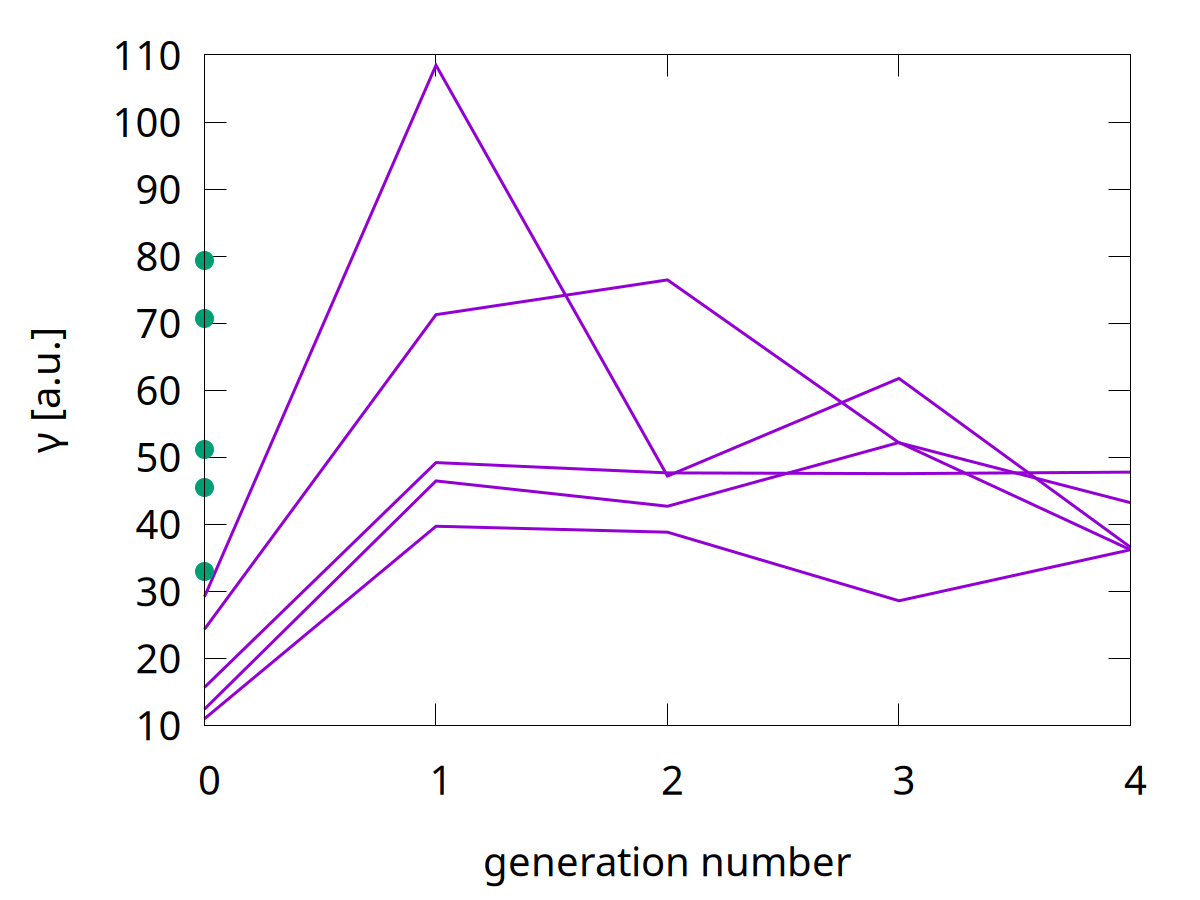
\includegraphics[width=.8\textwidth]{Pics/stats/gen-G.png}
        \caption{} \label{fig:emma-G-gen}
    \end{subfigure}
    \begin{subfigure}{.45\textwidth}
        \centering
        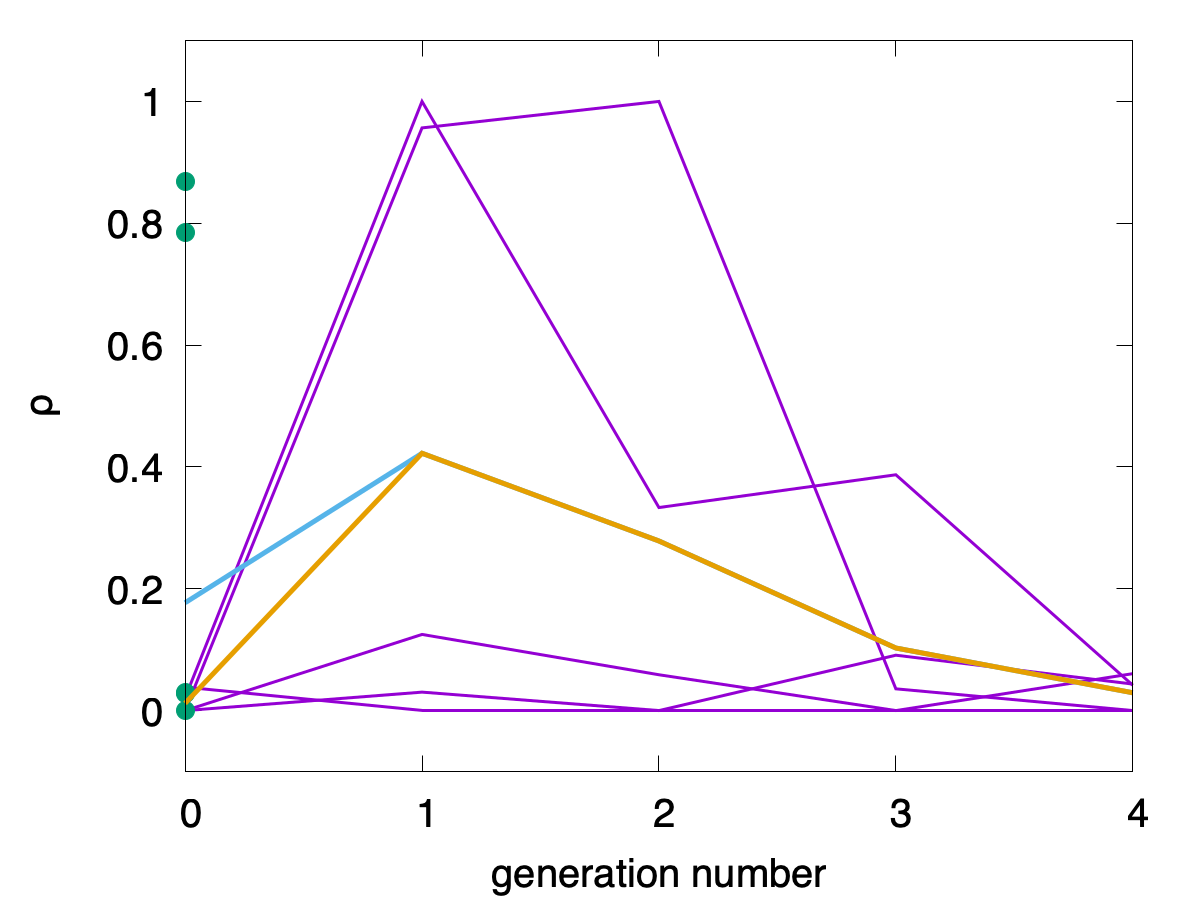
\includegraphics[width=.8\textwidth]{Pics/stats/gen-phd.png}
        \caption{} \label{fig:emma-phd-gen}
    \end{subfigure}
    \caption{Each $\gamma$ (a) and $\rho$ (b) of each particle and each generation after initial selection process} 
    \label{fig:emma-gen}
\end{figure}

%%% EQUATION 
Equations \ref{eq:emma-G3}-\ref{eq:emma-vcal3} and \ref{eq:emma-G4}-\ref{eq:emma-vcal4} represent the prediction functions at $t=3$ and $t=4$ rounded to 2 significant digits, respectively.
$h(x)$ is the hinge function (also called a rectifier function) of the simple form $h(x) = max(0,x)$. 
The expression $h(\lambda-6)$ translates into layer count only has an influence if larger than 6 
and $h(6-\lambda)$ into layer count influential only if under 6.
%
The first thing to notice is that every prediction function of a generation depends on the same variables. 
%This means that the algorithm must decide on the variables which explain the most variance independent of optimization weights.
This stems from the fact that the algorithm must chose a single minimal set of basis functions to predict all dependent variables. 
%
Knowing this, makes the decision of adding $\lambda$ and $v_{cal}$ as dependent variables rather unfortunate. %highly questionable. 
%As the \gls{mars} algorithm is gready,
Different independent variables compete to be in the prediction functions because of the greediness of the \gls{mars} algorithm. 
%\td{This makes including $\lambda$ and $v_{cal}$ as dependent variables unfortunate decisions with hindsight.}
In equations \ref{eq:emma-phd3} and \ref{eq:emma-G3} the coefficient have the same signs and differ by a factor of roughly 100.
This fits the data well, but the positive influence of the layer count/number is counter intuitive 
as one would expect more layers to be more insulating and thus result in lower conductance and a lower probability of pin holes going all the way trough the \gls{zro} layer. %pin hole density. 
The coefficients of the $v_{cal} \cdot T_{cal}$ interaction in equations \ref{eq:emma-phd3} and \ref{eq:emma-G3} 
seem low, but considering the minimum value of the inter action of \num{36000} should not be under estimated. 
%It's positive the hinge
It is astonishing that the knot of the hinge function for equations \ref{eq:emma-phd3}-\ref{eq:emma-vcal3} was chosen so low; 
basically only including the influence of $\lambda=4$.
On the positive site the calcination heating rate $v_{cal}$ (see equation \ref{eq:emma-vcal}) has been predicted perfectly within numerical precision. 

For each generation the \gls{mse} was calculated such that only samples were used which were available at that time. 
It is 64, 158, 54 and 50 for $t=1,2,3,4$, respectively. 
The high \gls{mse} can be explained because the prediction function is only a constant at $t=2$. 
Appart from the second generation the \gls{mse} falls over time, which might be attributed to overfitting.
The \gls{mse} for each generation was calculated between predicted values for pre-optimisation samples to check for overfitting, 
but the the error sank with each generation (except for the second gen): 102, 118, 58, 50, respectively for $t=1,2,3,4$. 

It is interesting that although prediction functions for $t=3$ perfectly predicted $v_{cal}$ 
the combined \gls{mse} for $t=4$ is lower. 
%%% MAIN INFLUENCE 
%Even without considering the large maximum of $T_{cal}$, 

\iffalse
The coefficient for $T_{cal}$ is the largest for all equations. 
Factoring in the large maximum value of $T_{cal}$ in contrast the other independent variables, 
$T_{cal}$ has the by far the largest influence on the dependent variables. 
The coefficient of the interaction of $layr$ and $T_{cal}$ is about a tenth in size, %interaction between?H
but has the extra factor of $layr$ of up to 12, resulting in the products being in the same order of magnitude.
I can be noted that the coefficient of the $layr\cdot T_{cal}$ interaction always has contrary sign to $T_{cal}$ coefficient. 
%%% EXPECTATION
It should be doubted, though, that the $layr$ only appears as interaction term 
together with $T_{cal}$ and $T_{DB}$, which seems rather than an artefact. 
\fi

\begin{align}
%
%    \label{eq:emma-phd1}
%    \hat{\rho}_1 &= -26  + 0.0025 \cdot T_{DB}\cdot T{Cal}  +  0.056 \cdot  h(6-\lambda)\cdot T_{Cal} \\
%    \label{eq:emma-G1}
%    \hat{\gamma}_1 &= -0.52 + 2.3\cdot 10^{-5} \cdot  T_{DB}\cdot T_{Cal} + 0.00080 \cdot h(6-layr)\cdot T_{cal}\\
%    \label{eq:emma-layr1}
%    \hat{\lambda}_1 &= 7.1 + 8.1\cdot 10^{-5} \cdot T_{DB}\cdot T_{cal} -  0.0056 \cdot  h(6-layr)\cdot T_{cal}\\
%    \label{eq:emma-vcal1}
%    \hat{v}_{cal,1} &= 19 - 0.00025 \cdot  T_{DB}\cdot T_{cal} - 0.0055 \cdot  h(6-layr)\cdot T_{cal}\\
%
%    \label{eq:emma-phd2}
%    \hat{\rho}_2 &= 47\\
%    \label{eq:emma-G2}
%    \hat{\gamma}_2 &= 0.23\\
%    \label{eq:emma-layr2}
%    \hat{\lambda}_2 &= 7.3\\
%    \label{eq:emma-vcal2}
%    \hat{v}_{cal,2} &= 10\\
%
    \label{eq:emma-phd3}
    \hat{\rho}_3 &= 0.075  -   0.0014 \cdot  v_{cal}  +    0.18 \cdot  h(6-\lambda)  + 3.9\cdot 10^{-06} \cdot  v_{cal}\cdot T_{cal} \\
    \label{eq:emma-G3}
    \hat{\gamma}_3 &= 43  -   0.097 \cdot  v_{cal}  +     10 \cdot  h(6-\lambda)  + 0.00026 \cdot  v_{cal}\cdot T_{cal} \\
    \label{eq:emma-layr3}
    \hat{\lambda}_3 &= 9.9  - 0.00064 \cdot  v_{cal}  -     2.7 \cdot  h(6-\lambda)  - 1.3\cdot 10^{-06} \cdot  v_{cal}\cdot T_{cal} \\
    \label{eq:emma-vcal3}
    \hat{v}_{cal,3} &= -5.2\cdot 10^{-15}  +   0.016 \cdot  v_{Cal}  + 1.3\cdot 10^{-15} \cdot  h(6-\lambda)  + 3.9\cdot 10^{-21} \cdot  v_{Cal}\cdot T_{cal} \\
%
    \label{eq:emma-phd4}
    \hat{\rho}_4 &=  -0.87 + 0.0047 \cdot  T_{cal} - 0.00036 \cdot  \lambda\cdot T_{cal}  +  0.0024 \cdot  h(\lambda-6)\cdot T_{DB} \\
    \label{eq:emma-G4}
    \hat{\gamma}_4 &=     -19 + 0.28 \cdot  T_{cal}  - 0.022 \cdot  \lambda\cdot T_{cal}  +  0.16 \cdot  h(\lambda-6)\cdot T_{DB} \\
    \label{eq:emma-layr4}
    \hat{\lambda}_4 &=  6.8 - 0.014 \cdot  T_{cal}  + 0.0018 \cdot  \lambda\cdot T_{cal}  + 0.0060 \cdot  h(\lambda-6)\cdot T_{DB} \\
    \label{eq:emma-vcal4}
    \hat{v}_{cal,4} &=  29 - 0.052 \cdot  T_{cal}  + 0.0011 \cdot  \lambda\cdot T_{cal}  -  0.011 \cdot  h(\lambda-6)\cdot T_{DB} 
\end{align}
%\fi
%what was the best result? For each particle there is best and global best. 

%The calcination heating $v_{cal}$ rate has been predicted perfectly. 
%\td{even though $v_{cal}$ doesn't appear in the prediction function, how is this possible?}
%The number of layers $\lambda$ on the other hand was predicted poorly 
%even though the conversion factor was $1$ and the prediction function dependent on $\lambda$. 


%%%%%%%%%%%%%%%%%%%%%%%%%%%%%%%%%%%%%%%%%%%%%%%%%%%%%%%%%%%%%%%%%%%%%%%%%%%%%%%%%%%%%%%%5
%\subsubsection{how did evolve over time?}


%\iffalse
%\fi

\iffalse
\begin{figure}
\centering
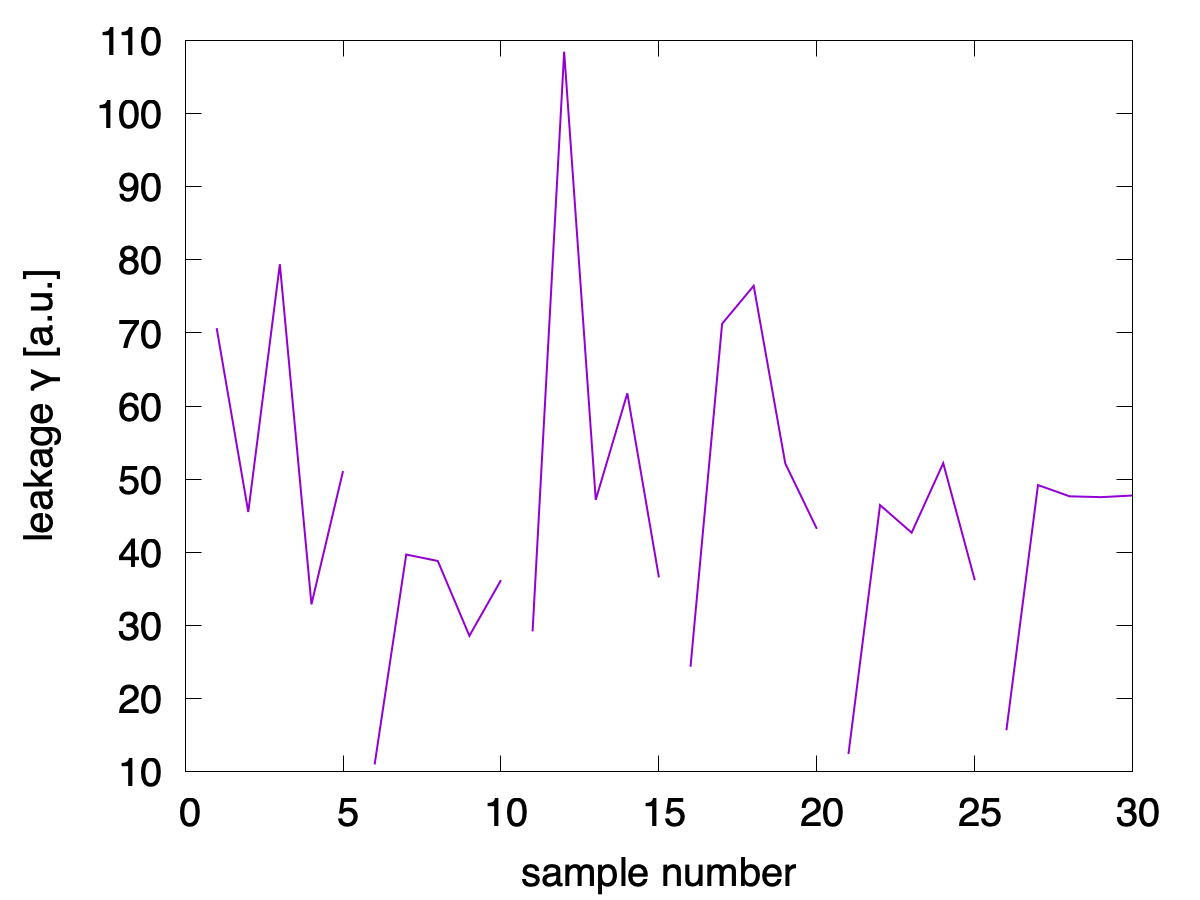
\includegraphics[width=.6\textwidth]{Pics/stats/G-t.png}
    \caption{conductivity G [a.u.] against sample number (is this even correct?)}
    \label{fig:G-t}
\end{figure}

\td{TODO: check if the sorted correctly? Make generation graph with boxplot }
\td{TODO: visualize} how the population moved across the space (with parallel coordinates? or see page 121)
\url{https://stackoverflow.com/questions/30228281/gnuplot-parallel-coordinates-axes-plot-key-annotation}
\fi

%%%%%%%%%%%%%%%%%%%%%%%%%%%%%%%%%%%%%%%%%%%%%%%%%%%%%%%%%%%%%%%%%%%%%%%%%%%%%%%%%%%%%%%%5
%\subsubsection{what is best}
%%%%%%%%%%%%%%%%%%%%%%%%%%%%%%%%%%%%%%%%%%%%%%%%%%%%%%%%%%%%%%%%%%%%%%%%%%%%%%%%%%%%%%%%5
\subsubsection{influence of variable selection on outcome}
The heating rate of the calcination process $v_{cal}$ and the number of layers $\lambda$ were included as dependent variable with the objective to maximize with a relative weight of 0.05 each.
The idea was to maximize $v_{cal}$ and minimize $\lambda$ in order to minimize the process time. 
Another thought behind including $v_{cal}$ and $\lambda$ was to test if the algorithm would correctly predict those. 
%
Three major flaws behind this consideration became obvious with time: 
%
\todo{
(1) The true function for predicting $v_{cal}$ and $\lambda$ are $v_cal*60$ ($C/h$ instead of $C/min$) and $\lambda$, respectively. 
The algorithm will tend to include those values into the prediction function for 
all dependent variables and possibly exclude others which have more influence 
on $\gamma$ and $\rho$ (see equations \ref{eq:emma-G} and \ref{eq:emma-phd}).
%
(2) The algorithm would be influenced by those values to choose samples, which potentially optimize $v_{cal}$ and/or $\lambda$ but not $G$ or $\rho$. 
%
(3) needlessly making the problem more complicate %, important time (around 10\% of the samples) could have been replaced with more insightful samples. 
\begin{itemize}
    \item MARS chooses same set from independent variables for predicting all dependent variables. 
    \item flaws of MARS: all functions are dependent on same independent vars
    \item Every output var is independent of each other, so $v_{cal}$ can act as test 
heating rate was one of the dependent variables with the intention of minimizing the variable. 
It can also be used as test to see how well the EMMA performs (or rather, more precisely MARS)
It doesn't influence the fit for the other splines, but it influences the choice of samples therefore it might have slowed down the process
Overall there were too many variables involved for such a small dataset
        that means that adding dependent variables influences \td{previous variables}
\end{itemize}
}

\td{look at emma papers}
\td{change G to gamma and write enr to every figure}
\td{calculate MSE for predictions}

